\documentclass[12pt,a4paper]{article}
\usepackage{a4wide}

% ENCODING
\usepackage[T1]{fontenc}
\usepackage[utf8x]{inputenc}
\DeclareUnicodeCharacter{8656}{\ensuremath{\Leftarrow}}
\DeclareUnicodeCharacter{10214}{\ensuremath{\llbracket}}
\DeclareUnicodeCharacter{10215}{\ensuremath{\rrbracket}}
\DeclareUnicodeCharacter{8871}{\ensuremath{\models}}
\DeclareUnicodeCharacter{8614}{\ensuremath{{\mapsto}}}
\DeclareUnicodeCharacter{955}{\ensuremath{\lambda}}
\DeclareUnicodeCharacter{956}{\ensuremath{\mu}}
\DeclareUnicodeCharacter{957}{\ensuremath{\nu}}
\DeclareUnicodeCharacter{963}{\ensuremath{\sigma}}

\usepackage{graphicx}
\usepackage{xcolor}
\usepackage{MnSymbol}
\usepackage{stmaryrd}
\usepackage{amsthm}

\usepackage{array}
\newcolumntype{L}{>{$}l<{$}}
\newcolumntype{C}{>{$}c<{$}}
\newcolumntype{R}{>{$}r<{$}}

\theoremstyle{remark}
\newtheorem*{remark}{Remark}

% CODE LISTINGS
\usepackage{listings}
\lstset{
  language=C,
  columns=[l]fullflexible,
  mathescape=true,
  basicstyle=\ttfamily,
  commentstyle={}, 
  showstringspaces=false
} 

% SEPARATION LOGIC
\newcommand{\iterstar}[2][]{\circledast^{#1}_{#2}}
\renewcommand{\bigstar}{\circledast}
\newcommand{\magicwand}{\mathbin{{-\!\!}{*}}}
\newcommand{\septract}{\mathbin{{-\!}{\circledast}}}
\newcommand{\Pto}[1][]{\stackrel{\mbox{\scriptsize \smash{$#1$}}}\mapsto}
\newcommand{\pto}[1][]{{\Pto[#1]}}
\newcommand{\halfpto}{\pto[.5]}
\newcommand{\combine}{\mathop{\hspace{-1pt}\cdot\hspace{-1pt}}}

\newcommand{\checkthis}{$^{\rm [check\ this]}$}
\newcommand{\floor}[2][]{\left\lfloor{#2}\right\rfloor_{#1}}
\newcommand{\ceil}[2][]{\left\lceil{#2}\right\rceil_{#1}}
\newcommand{\floorpow}[1]{\llfloor{#1}\rrfloor}
\newcommand{\fracpow}[1]{\{\hspace{-3pt}\{{#1}\}\hspace{-3pt}\}}

\newcommand{\setC}{\raisebox{1.5pt}{$\blacktriangledown$}}
\newcommand{\unsetC}{\raisebox{1.5pt}{$\triangledown$}}
\newcommand{\setP}{{\blacktriangle}}
\newcommand{\unsetP}{{\triangle}}

% BIT OPERATIONS
\newcommand{\AND}{\mathbin{\texttt{\&}}}
\newcommand{\OR}{\mathbin{\texttt{|}}}
\newcommand{\NOT}{\mathbin{\textasciitilde}}
\newcommand{\SHIFTRIGHT}{\mathbin{\texttt{>}\hspace{-1pt}\texttt{>}}}
\newcommand{\SHIFTLEFT}{\mathbin{\texttt{<}\hspace{-1pt}\texttt{<}}}

\title{An explanation of Doug Lea's memory manager}
\author{John Wickerson}
\date{}

\begin{document}

\maketitle

\begin{abstract}
We describe the basic functionality of Doug Lea's memory manager.
\end{abstract}

\section{The routines}

There are four main public routines:

\begin{itemize}
\item {\tt malloc($n$)} returns a pointer to a newly-allocated chunk with payload at least $n$ bytes, or {\tt null} if no space is available. It uses the internal {\tt chunk\_alloc} routine.
\item {\tt free($p$)} releases the chunk identified by $p$, and has no effect if $p$ is {\tt null}. It uses the internal {\tt chunk\_free} routine.
\item {\tt realloc($p$, $n$)} returns a pointer to a chunk with payload at least $n$ bytes, that contains the first $n$ bytes of data in $p$ (or all of it if it has fewer than $n$ bytes of payload), or {\tt null} if no space is available. The pointer returned may or may not be the same as $p$. We do not plan to verify this routine.
\item {\tt calloc} is the same as {\tt malloc}, except the payload of the returned chunk is fully zeroed. We do not plan to verify this routine.
\end{itemize}

\section{The arena and boundary tags}

\begin{figure}[tbhp]
\centering{
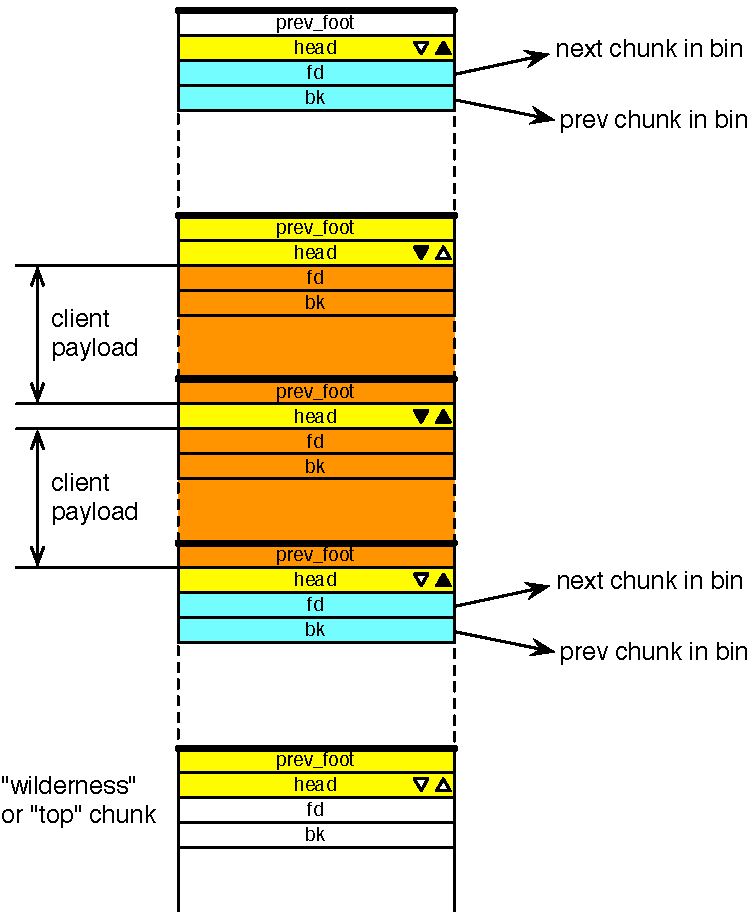
\includegraphics{dlmalloc_arena.pdf}
}
\caption{The arena}
\label{fig:arena}
\end{figure}

The arena is shown in Fig.~\ref{fig:arena}. The ``blocks'' of the Unix V7 memory manager are now called ``chunks''. The layout of these chunks evolves over time as they are allocated, freed, split and coalesced. The procedures ensure that no free chunk ever borders another free chunk -- these would always be coalesced. Boundary tags (as first described by Knuth in 1973) are used to simply this
coalescing: each chunk stores its own size and the size of its predecessor (in the {\tt head} and {\tt prev\_foot} fields respectively), which effectively makes the arena into a doubly-linked list. Put concretely: given a pointer {\tt p} to a chunk, the addresses of the previous and next chunks can be computed as follows:
\begin{lstlisting}
prev_chunk(p) = (mchunk *)(((char *)p) - (p -> prev_foot))
next_chunk(p) = (mchunk *)(((char *)p) + ((p -> head) & ~111$_b$))
\end{lstlisting}

The divisions between chunks are highlighted with thick black lines. See how the payload of an in-use chunk actually overlaps the {\tt prev\_foot} field of the next chunk. This is fine: the next chunk doesn't need to able to reach the in-use chunk until the in-use chunk becomes free. Upon becoming free, the {\tt prev\_foot} field can be recalculated.

\subsection{Flags}

Chunks are 8-byte aligned, so the three lowest order bits of the {\tt head} field are redundant. The two lowest are employed as flags; the third-lowest is ``not used by this malloc, but might be useful in extensions''. It is impossible for both the previous and the current blocks to be free (they would have already been coalesced), so the fourth configuration in Table~\ref{tab:flags} is used to signify that the block is memory mapped (see \S\ref{sect:memory_mapping}).
\begin{table}
\centering{
\begin{tabular}{cc|l}
{\tt CINUSE} & {\tt PINUSE} & interpretation \\ \hline
0 & 1 & previous chunk is in use, current block is free \\
1 & 0 & previous chunk is free, current block is in use \\
1 & 1 & both previous and current blocks are in use \\
0 & 0 & current block is memory mapped
\end{tabular}
}
\caption{The flags in each chunk's {\tt head} field}
\label{tab:flags}
\end{table}
In Fig.~\ref{fig:arena}, the downwards-pointing triangle refers to the current chunk, while the upwards-pointing triangle refers to the previous chunk. A filled triangle denotes a set bit.

\begin{remark}Interestingly, this interpretation was changed in the 2009 release. Previously, the lowest bit stored whether or not the previous chunk was in use, and the second-lowest stored whether or not the current chunk was memory mapped. This meant that to determine whether the current chunk was in use, one had to look at the {\tt prev\_foot} field of the \emph{next} chunk!
\end{remark}

Note that {\tt PINUSE} is permanently set for the first chunk in the arena, so as to avoid attempts to coalesce with non-existant memory.

\subsection{The top chunk}\label{sect:the_top_chunk}

The last chunk in the arena is called the top chunk, or the wilderness chunk. It is always free, and its size is defined to be bigger than any other chunk, since it can almost always be made so via a call to {\tt sbrk}. This way, it is only used when no other chunk is big enough, and we thus avoid unnecessary {\tt sbrk} calls. Page 39 of the source code comments that ``the actual size of [the] topmost space is {\tt topsize}+{\tt TOP\_FOOT\_SIZE}, which includes space reserved for adding fenceposts and segment records if necessary when getting more space from the system.''

\subsection{Bin pointers}

The {\tt fd} and {\tt bk} fields locate the chunk within a second datastructure called a bin, which is essentially a circular linked-list comprising chunks of the same or a similar size. The fields are overwritten when the chunk is allocated, and hence are only used by free chunks. Because each chunk has these four 4-byte fields, the minimum chunk size is 16 bytes -- that is, {\tt malloc(0)} allocates a chunk of 16 bytes.

\section{Binning}\label{sect:binning}

Free chunks are maintained in bins, which are circular doubly-linked lists of chunks of the same or similar size. Free chunks whose size is a multiple of 8 bytes up to 248 bytes are stored in one of 32 ``small'' bins that link identically-sized chunks. Chunks of 256 bytes or more are stored in one of 32 ``tree'' bins. 

Initially, all of the bins are empty, because at the start the whole heap is composed of one single chunk, the wilderness chunk, which is never included in any bin.

\subsection{Small bins}\label{sect:small_bins}

A chunk of size $n$ bytes is stored in the bin at array index
$\floor{n/8}$. Since the smallest chunk size is 16 bytes, the first
two bins seem to be redundant\checkthis. There is something a little
funny here: the variable {\tt NSMALLBINS} is set to 32, but the array
{\tt smallbins} has $({\tt NSMALLBINS}+1) × 2 = 66$ elements.

\subsection{Tree bins}\label{sect:tree_bins}

There are 32 more bins, which have ranges that increase approximately logarithmically. The maximum chunk size that can be accommodated is about 2 GB. Chunks are sorted by size within each bin. All free chunks are binned, except the remainder of the most recently split chunk (called the designated victim) and the top chunk.

Suppose a chunk has size $n$ bytes. The {\tt compute\_tree\_index} macro is responsible for calculating the appropriate index $I$ into the array of tree bins. If $n$ is less than 256 bytes, then $I$ is 0 (although in such a case, the {\tt compute\_tree\_index} macro wouldn't be used: the chunk would be in a small bin). If $n$ is greater than FFFFFF$_h$ then $I$ is the
last index in the array: ${\tt NTREEBINS} - 1$\footnote{Not sure why the upper limit is FFFFFF.}. In general, $I$ is defined as follows:
\[
I = \left\{\begin{array}{ll}
0 & \text{if } n < 2^8 \\
{\tt NTREEBINS} - 1 & \text{if } n ≥ 2^{24} \\
2(\floor{\log_2 n}-8) & \text{if } \fracpow{n} < \floorpow{n}/2 \\
2(\floor{\log_2 n}-8) + 1 & \text{if } \fracpow{n} ≥ \floorpow{n}/2
\end{array}\right.
\]
where the $\floorpow{-}$ operator rounds its input down to the nearest power of two, that is: $\floorpow{n} = 2^{\floor{\log_2{n}}}$. We also define $\fracpow{n} = n - \floorpow{n}$, notationally recalling the $\{-\}$ operator from arithmetic, which returns the fractional part of a real number. Note that for all $n>0$, $\fracpow{n}$ must always lie between 0 (inclusive) and $\floorpow{n}$ (exclusive). The last two clauses in the definition above pivot upon the median of this range, thus yielding two equally-spaced bins for each power of two. The offset 8 is required because the tree bins only begin at chunk sizes of $2^8$ bytes. To clarify, the ranges of each tree bin are as follows. Note that all numbers are written in hexadecimal.
\[
\begin{tabular}{l|l}
Size $n$ in hex (bytes) & Bin index \\ \hline
$100 ≤ n < 180$ & 0 \\
$180 ≤ n < 200$ & 1 \\
$200 ≤ n < 300$ & 2 \\
$300 ≤ n < 400$ & 3 \\
$400 ≤ n < 600$ & 4 \\
$600 ≤ n < 800$ & 5\\
\vdots & \vdots
\end{tabular}
\]

\subsection{Memory mapping}\label{sect:memory_mapping}
Page 34 of the source code explains that the {\tt prev\_foot} field of a memory-mapped chunk is used to hold the chunk's offset within its memory mapped region. This is needed to preserve alignment. Each memory-mapped chunk is trailed by the first two fields of a fake next chunk, for the sake of usage checks.

\section{Outline of {\tt dlmalloc}}

The algorithm runs roughly as follows:

\lstset{basicstyle=\small\sffamily, commentstyle={}, numbers=left, stepnumber=5, xleftmargin=7.5mm, numberstyle=\tiny}
\begin{lstlisting}
void* dlmalloc(size_t bytes) {
   if bytes $≤$ MAX_SMALL_REQUEST
      if a smallbin of the right size is non-empty
         return a chunk from that smallbin
      else if designated victim is not big enough
         if there exists a non-empty sufficiently-large smallbin
            return (first part of) chunk from smallest such smallbin
         else if there exists a non-empty treebin
            if allocation in a treebin succeeds, return the resulting chunk
   else if bytes $≥$ MAX_REQUEST, return fail 
   else // MAX_SMALL_REQUEST < bytes < MAX_REQUEST
      if allocation in a treebin succeeds, return the resulting chunk
   // either the designated victim is big enough,
   // or all bins are empty, or treebin allocation failed
   if designated victim is big enough
      return (first part of) designated victim
   else if top chunk is big enough
      return (first part of) top chunk
   try to obtain the memory from the system
}
\end{lstlisting}

The above presentation is, however, quite hard to follow because of the combination of nested conditionals with multiple return points. A clearer presentation is given by the flowchart in Fig.~\ref{fig:dlmalloc_flow}.

\begin{figure}
\centering{
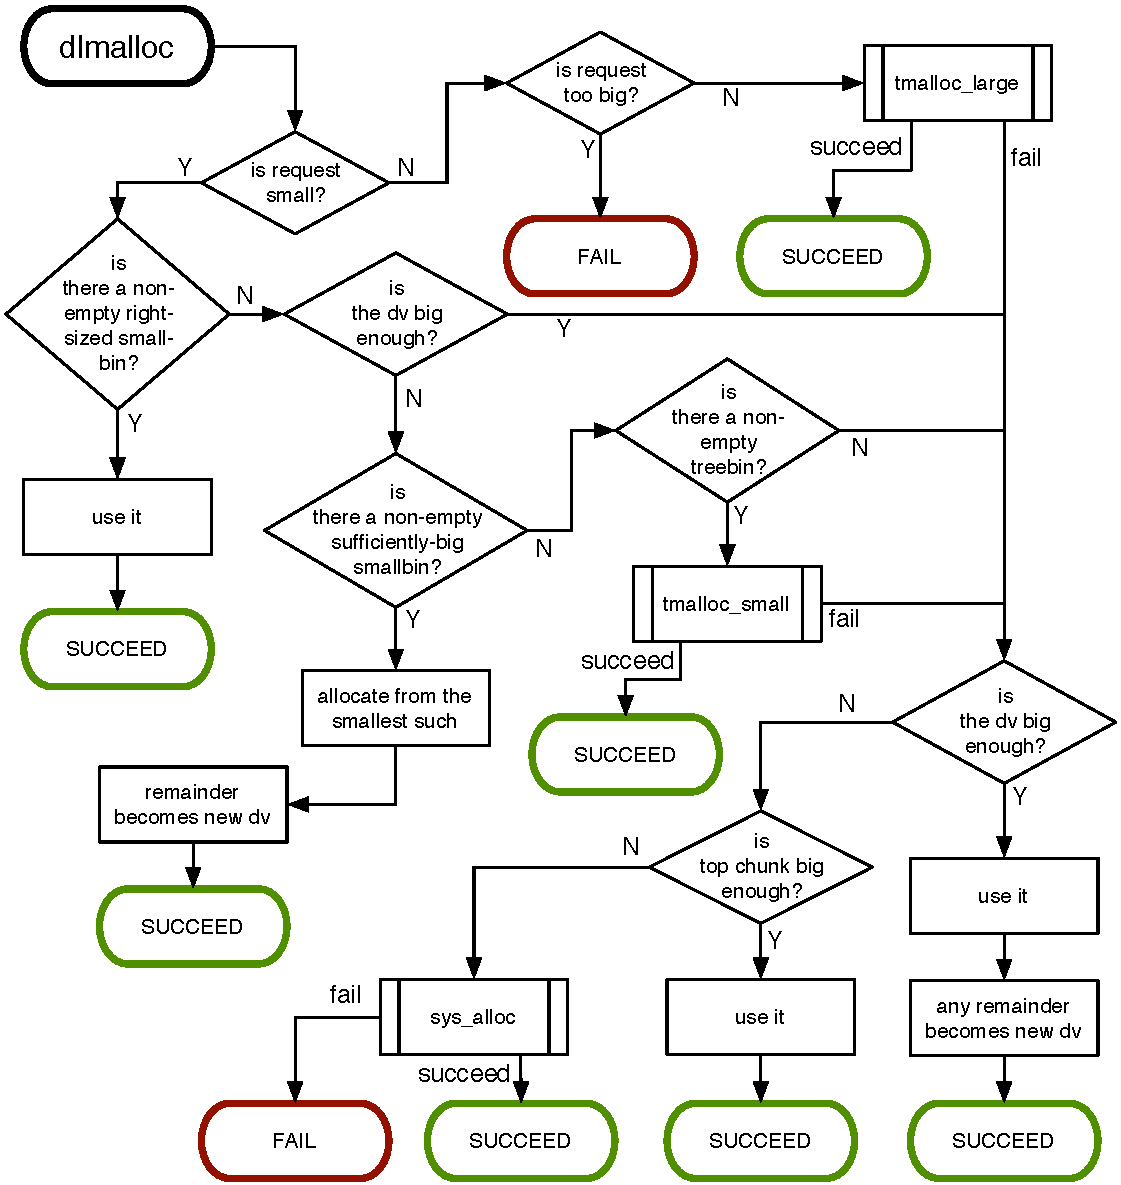
\includegraphics[width=\textwidth]{dlmalloc_flow.pdf}
}
\caption{Flowchart for {\tt dlmalloc}}
\label{fig:dlmalloc_flow}
\end{figure}

\section{Description of the state}

First define:
\[
\begin{array}{rcl}
p.\setC &⇔& p.{\tt head} \SHIFTRIGHT 1 \AND 1 \\
p.\unsetC &⇔& ¬(p.\setC) \\
p.\setP &⇔& p.{\tt head} \AND 1 \\
p.\unsetP &=& ¬(p.\setP) \\
p.CP &=& p.C ∧ p.P \qquad ∀C∈\{\setC,\unsetC\}, P∈\{\setP,\unsetP\} \\
p.size &=& p.{\tt head} \AND \NOT 3 \\
p→q    &=& p + p.size = q \\
p←q   &=& b.\unsetC ⇒ (q - q.{\tt prev\_foot} = p)\\
↔     &=& →∩← \\
↔^*, ←^*, →^*   &=& \text{reflexive transitive closures of } ↔,←, → \\
\end{array}
\]

The internal state of the memory manager comprises the arena plus several state state variables.
\[
\text{Overall state = } \boxed{mstate * arena}
\]
Where $mstate$ comprises:
\begin{itemize}
\item {\tt start}: an auxiliary variable added in for the purposes of the proof. Identifies the first chunk in the arena.
\item {\tt dv}, {\tt dvsize}: {\tt dv} identifies an arena chunk, and {\tt dvsize} its size. Define 
\[
dvOK ⇔ ({\tt dv}=0 ∧ {\tt dvsize}=0) ∨ ({\tt start}→^*{\tt dv} ∧ {\tt dv}.size = {\tt dvsize}).
\]
\item {\tt top}, {\tt topsize}: {\tt top} identifies the topmost arena chunk, and {\tt topsize} its size. See the remark in §\ref{sect:the_top_chunk} about {\tt topsize}. Define 
\[
topOK ⇔ {\tt start}→^*{\tt top} ∧ {\tt top}.size = {\tt topsize}.
\]
\item {\tt smallbins}: an array of smallbins. Note that the array has size 66, yet it holds only 32 smallbins. Define 
\[\begin{array}{c}
smallbin(i) = {\tt smallbin}[2i]\\
smallbinsOK ⇔ ∀i∈[0,32)\ldotp smallbinOK(smallbin(i)) \\
smallbinOK(b) ⇔ \text{``check that all chunks are free, in the arena, and the right size''.}
\end{array}\]
\item {\tt treebins}: an array of 32 pointers to treebins. Define 
\[\begin{array}{c}
treebinsOK ⇔ ∀i∈[0,32)\ldotp treebinOK({\tt treebins}[i]) \\ 
treebinOK(b) ⇔ \text{``check that all chunks are free, in the arena, and the right size''.}
\end{array}\]
\item {\tt smallmap}, {\tt treemap}: bit vectors that store whether each smallbin and treebin is empty or not. Define 
\[\begin{array}{c}
smallmapOK ⇔ ∀i∈[0,32)\ldotp {\tt smallmap}[i]=0 ⇔ smallbin(i)=∅\\
treemapOK ⇔ ∀i∈[0,32)\ldotp {\tt treemap}[i]=0 ⇔ treebin(i)=∅
\end{array}\]
\item {\tt least\_addr}: the least address ever obtained from {\tt sbrk} or {\tt mmap}. In contrast, {\tt start} is the least address ever obtained from {\tt sbrk} (I think).
\end{itemize}
So we can define $mstate$ like so:
\[
mstate = \begin{array}[t]{l} dvOK * topOK * smallbinsOK * treebinsOK {}\\{} * smallmapOK * treemapOK * {\tt least\_addr}↦5
\end{array}
\]

The $arena$ predicate can be defined like so:
\[
{\tt start} ↔^* {\tt top}
\]
This states that the arena is valid. The validity of the superimposed bin structure comes from the $smallbinsOK$ and $treebinsOK$ predicates. As for how to link a particular chunk to both its tree node and its arena node: this remains unclear for now.

\section{Outline of {\tt dlfree}}
\begin{figure}
\centering{
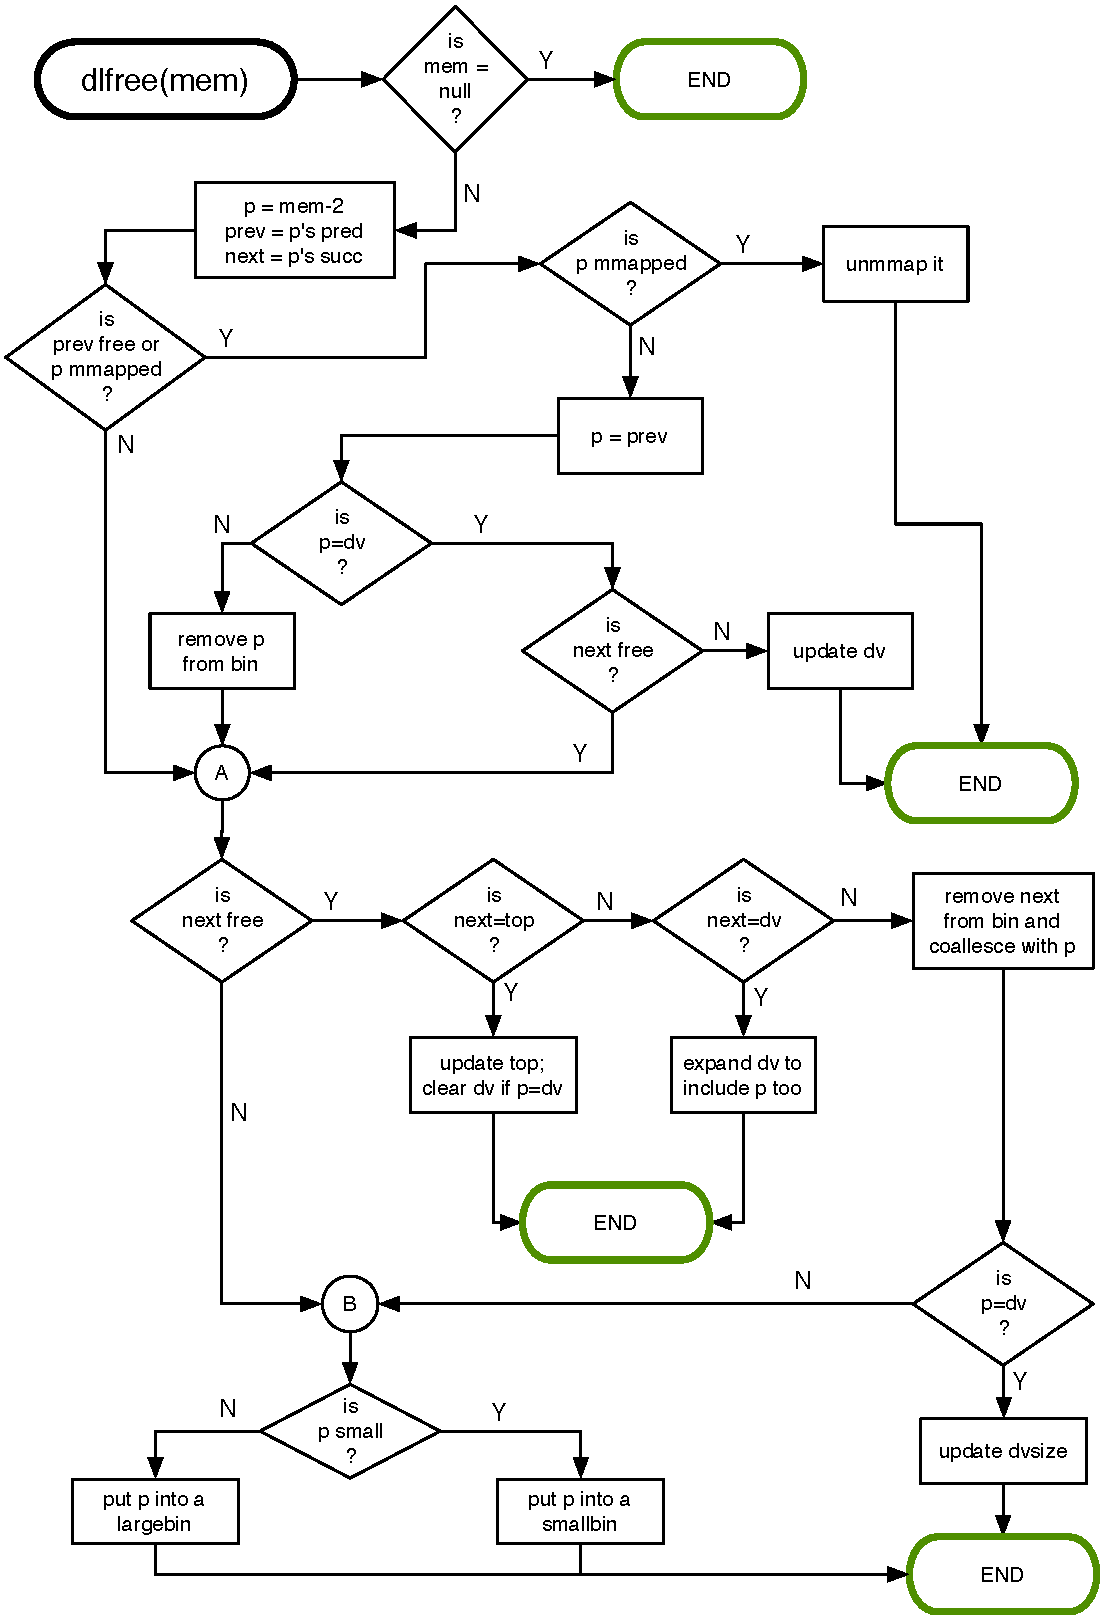
\includegraphics[height=0.95\textheight]{dlfree_flow.pdf}
}
\caption{Flowchart for {\tt dlfree}}
\label{fig:dlfree_flow}
\end{figure}

For a rough overview, see the flowchart in Fig.~\ref{fig:dlfree_flow}.


\end{document}